\documentclass[11pt]{article}

% 中文注释：ACL/EMNLP 投稿阶段建议使用 review 模式；定稿时可改回 \usepackage{acl}。
\usepackage[review]{acl}
\usepackage{times}
\usepackage{latexsym}
\usepackage[T1]{fontenc}
\usepackage[utf8]{inputenc}
\usepackage{microtype}
\usepackage{graphicx}
\usepackage{booktabs}
\usepackage{multirow}
\usepackage{amsmath}
\usepackage{amssymb}
\usepackage{natbib}
\usepackage{hyperref}
\usepackage{xcolor}
\usepackage{enumitem}
\usepackage{subcaption}
\usepackage{algorithm}
\usepackage{algorithmic}
\usepackage{pifont}
\newcommand{\cmark}{\ding{51}}
\newcommand{\xmark}{\ding{55}}

% 中文注释：为双栏排版增加少量断行弹性，尽量减少 underfull hbox 警告。
\emergencystretch=1.5em

\hypersetup{
    colorlinks=true,
    linkcolor=blue,
    citecolor=blue,
    urlcolor=blue
}

% 中文注释：按 ACL 字体要求，术语标记改为 Times 系正文样式，不再依赖等宽或粗体字形。
\newcommand{\eventmark}{\textcolor{blue}{event time}}
\newcommand{\recordmark}{\textcolor{red}{record time}}

% 中文注释：保留原题目语义，仅按 ACL 模板常见写法控制手工换行。
\title{BiTempQA: A Diagnostic Benchmark for Bitemporal Reasoning\\ in LLM Agent Memory Systems}

\author{
  Anonymous
}

\begin{document}
\maketitle
\begin{abstract}
Memory-augmented LLM agents must track not only \emph{what} happened but \emph{when} it happened and \emph{when they learned about it}, a dual-timestamp (bitemporal) distinction critical for real-world applications such as medical records, financial systems, and news analysis.
Existing benchmarks either ignore timestamps entirely or treat time as a single dimension, leaving a gap in evaluating this capability.

We introduce \textbf{BiTempQA}, a diagnostic benchmark of 415 Chinese question-answer pairs (84 held-out test, all sourced from real-world data) across 10 scenario types and 3 question types at two difficulty levels, where each memory entry carries explicit \texttt{event\_time} (when something occurred) and \texttt{record\_time} (when the system stored it) annotations.
Over half (56.0\%) of test questions require reasoning about both timestamps simultaneously.
The dataset combines ChronoQA news data (200 scenarios) with 15 manually curated real-world temporal event scenarios and 118 LLM-generated scenarios covering rare types (64.6\% real-source overall).
We evaluate seven memory backends (FAISS, BM25, Naive RAG, Simple KG, ChromaDB, Mem0, Graphiti) through a unified Retrieve$\to$LLM Generate$\to$LLM Judge pipeline with controlled evaluation parameters (same embedding model, same top-$k$, same generator).
We find that: (1) the top four lightweight systems are statistically indistinguishable (81.0--82.1\%, $p{>}0.3$), suggesting that retrieval design matters less than answer generation quality for short-context bitemporal scenarios; (2) ChromaDB's metadata filtering approach fails catastrophically (22.6\%) due to heterogeneous temporal formats in real-world data; (3) production memory systems (Mem0, Graphiti) dramatically underperform lightweight baselines, revealing that aggressive memory compression destroys bitemporal detail; and (4) real-world and LLM-generated scenarios yield comparable accuracy, validating our data augmentation approach.
BiTempQA is released as an open diagnostic tool for developing temporally-aware memory systems.

\end{abstract}

\section{Introduction}

\begin{figure*}[t]
\centering
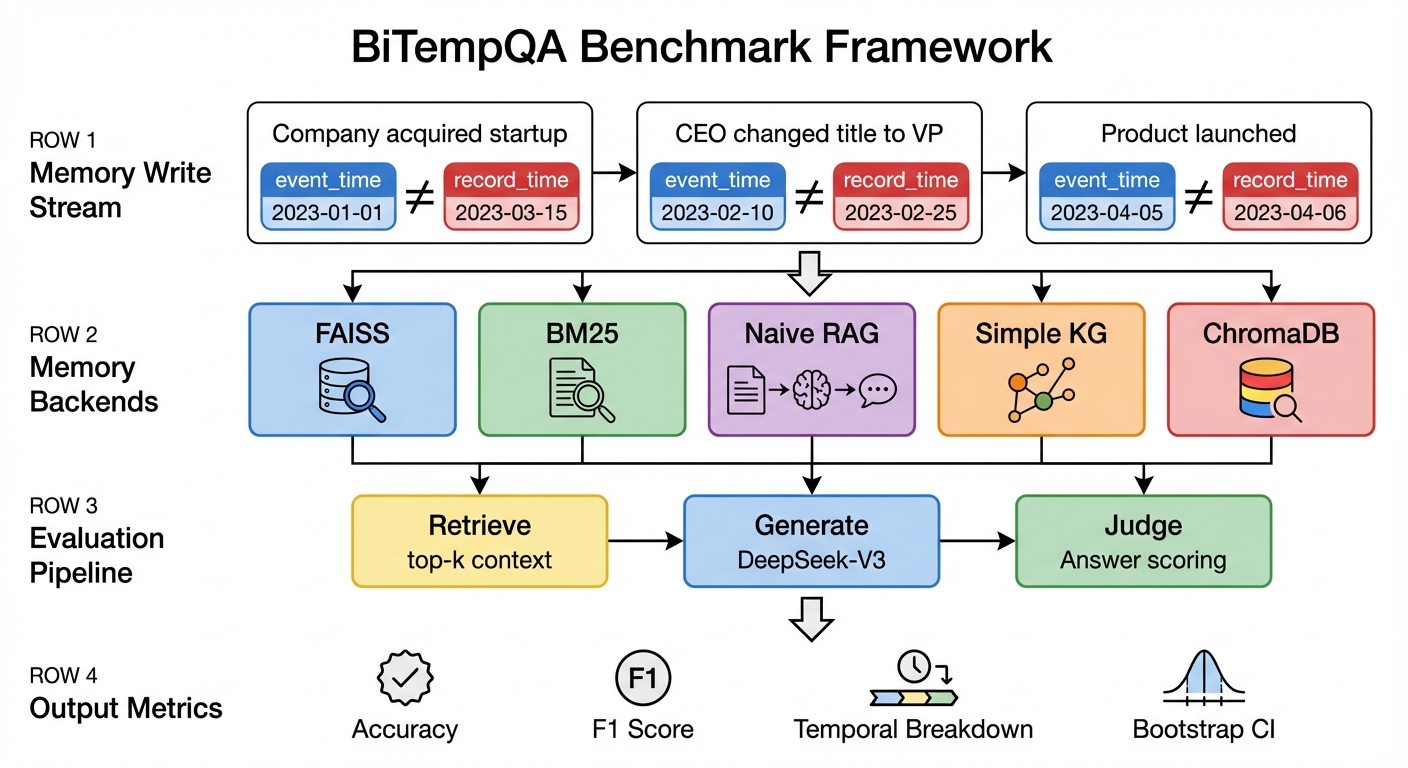
\includegraphics[width=\textwidth]{figures/fig1_framework.jpeg}
% 中文注释：caption 保留原意，但把语气调整得更自然、更符合论文写法。
\caption{BiTempQA framework overview. Each memory write carries dual timestamps: \textcolor{blue}{event time}, indicating when the event occurred, and \textcolor{red}{record time}, indicating when the system recorded it. Five memory backends retrieve context, which is then processed in a unified Retrieve $\rightarrow$ Generate $\rightarrow$ Judge pipeline to produce diagnostic metrics.}
\label{fig:framework}
\end{figure*}

Consider a medical AI assistant that learns at 10:00~AM on Tuesday that a patient's symptoms began two days earlier.
% 中文注释：这里保留必要斜体强调，但把举例句式改得更严谨，减少口语感。
To answer ``What was the patient's status on Sunday morning?'' correctly, the system must distinguish \emph{when the symptoms started} (event time) from \emph{when the system recorded this fact} (record time).
This bitemporal distinction, well established in temporal database theory~\citep{snodgrass1999tsql2,jensen1999temporal}, arises in many settings: financial trades execute on Monday but settle on Wednesday, news events occur on Thursday evening but are reported on Friday morning, and scientific findings may be established in 2022 but published in 2024.
A memory system that conflates these timestamps is therefore likely to make incorrect temporal inferences.

Despite its practical importance, this capability is not systematically evaluated in existing benchmarks for LLM-based memory systems.
Temporal reasoning benchmarks such as \textsc{TimE}~\citep{time2025}, \textsc{ETRQA}~\citep{etrqa2024}, and \textsc{Test of Time}~\citep{testoftime2025} primarily study reasoning over static text rather than over dynamically evolving memory stores.
Memory-system benchmarks such as LoCoMo~\citep{locomo2024}, LongMemEval~\citep{longmemeval2024}, and MemoryAgentBench~\citep{memoryagentbench2025} include temporal questions, but they generally treat time as a single dimension and do not distinguish event occurrence from information acquisition.
% 中文注释：把“我们无法诊断”改成更客观的“仍难以判断”，语气更符合学术论文。
As a result, it remains difficult to determine whether failures on temporal questions arise primarily from \emph{retrieval limitations} or \emph{reasoning limitations}, and which temporal reasoning types are most challenging.

We present BiTempQA, a diagnostic benchmark designed to address this gap.
BiTempQA is grounded in a central idea from bitemporal data modeling: each fact has two independent temporal dimensions.
% 中文注释：这里收紧数据介绍的语气，同时保留所有原始统计信息不变。
The benchmark contains 1,536 Chinese QA pairs, including a 308-item held-out test set, spanning 10 scenario types across 6 domains, with 9 question types at 3 difficulty levels.
Each memory write carries explicit event-time and record-time annotations, and 56.5\% of questions require reasoning about both timestamps simultaneously.
We evaluate five memory backends (FAISS, BM25, Naive RAG, Simple Knowledge Graph, and ChromaDB) in a unified Retrieve $\rightarrow$ Generate $\rightarrow$ Judge pipeline.

Our contributions are as follows.
First, we introduce, to our knowledge, the first dual-timestamp diagnostic benchmark for memory systems, with explicit event-time and record-time annotations on every memory write and structured metadata on every question.
% 中文注释：这里把 claim 改成更可辩护的学术语气，避免把统计关联直接写成过强结论。
Second, we show that record-time reasoning is associated with lower accuracy than event-time reasoning ($p = 0.023$ in a mixed-effects regression controlling for question type, difficulty, and scenario), supporting the benchmark's diagnostic usefulness.
Third, we report several diagnostic findings: sampled failures appear primarily retrieval-related ($\sim 55\%$), confidence is often poorly calibrated (AUROC $< 0.5$ for some systems), and memory backends exhibit substantial complementarity (oracle +9.8pp over the best single system).
Fourth, we compare BiTempQA with LoCoMo~\citep{locomo2024} and find that graph-based memory is relatively strong on adversarial robustness (97.5\%) but comparatively weak on temporal reasoning (37.5\%).

\section{Related Work}

\subsection{Temporal Reasoning Benchmarks}
Recent years have seen a proliferation of temporal reasoning benchmarks for LLMs.
\textsc{TimE}~\citep{time2025} provides 38,522 questions across 11 subtasks at 3 difficulty levels, evaluating LLMs' ability to understand temporal expressions and reason about event sequences.
\textsc{ETRQA}~\citep{etrqa2024} consolidates event temporal reasoning datasets for reading comprehension.
\textsc{Test of Time}~\citep{testoftime2025} generates synthetic temporal reasoning tasks.
\textsc{MusTQ}~\citep{mustq2024} evaluates multilingual temporal KGQA across 10 languages.
However, all treat time as a \emph{single} dimension: none systematically distinguish event occurrence time from information recording time, a distinction critical for memory systems.

\subsection{Memory System Benchmarks}
The emergence of memory-augmented LLM agents has driven benchmark development.
LoCoMo~\citep{locomo2024} (ACL 2024) evaluates long conversational memory with 1,986 questions across 5 types, including adversarial and temporal categories.
LongMemEval~\citep{longmemeval2024} provides 4,500 questions testing 8 memory systems on single-hop, multi-hop, and temporal reasoning.
MemoryAgentBench~\citep{memoryagentbench2025} focuses on multi-dataset agent memory evaluation.
While these benchmarks include temporal questions, they do not systematically test \emph{dual-timestamp} reasoning, the ability to distinguish ``when this happened'' from ``when I learned about it.''

\subsection{Bitemporal Data Modeling}
The distinction between event time (valid time) and record time (transaction time) is foundational in temporal database research~\citep{snodgrass1999tsql2,jensen1999temporal}.
Bitemporal data models track both dimensions, enabling queries like ``what did the system know at time $T_1$ about events that occurred at time $T_2$?''
This concept has been extensively studied in database systems but has not been applied to evaluate LLM memory systems.
BiTempQA bridges this gap by bringing bitemporal reasoning into the memory system evaluation paradigm.

\subsection{Positioning}
Table~\ref{tab:benchmark_comparison} positions BiTempQA relative to existing work.
BiTempQA is the \emph{only} benchmark that (1) evaluates dual-timestamp reasoning and (2) tests multiple memory system backends.

\begin{table}[t]
\centering
\resizebox{\columnwidth}{!}{%
\begin{tabular}{lcccccc}
\toprule
\textbf{Benchmark} & \textbf{Year} & \textbf{Temp.} & \textbf{Dual TS} & \textbf{Mem} & \textbf{Lang} & \textbf{Scale} \\
\midrule
LoCoMo & 2024 & Partial & \xmark & \cmark & EN & 1,986 \\
LongMemEval & 2024 & \xmark & \xmark & \cmark & EN & 4,500 \\
TimE & 2025 & \cmark & \xmark & \xmark & EN & 38,522 \\
ETRQA & 2025 & \cmark & \xmark & \xmark & EN & Consol. \\
Test of Time & 2025 & \cmark & \xmark & \xmark & EN & Novel \\
MusTQ & 2024 & \cmark & \xmark & \xmark & Multi & 15K \\
\midrule
\textbf{BiTempQA} & \textbf{2026} & \cmark & \cmark & \cmark & ZH & 1,536 \\
\bottomrule
\end{tabular}%
}
\caption{Comparison with related benchmarks. \textbf{Dual TS}: evaluates dual-timestamp reasoning. \textbf{Mem}: tests memory backends (not just LLMs).}
\label{tab:benchmark_comparison}
\end{table}

\section{BiTempQA Benchmark}

\subsection{Problem Formulation}
Following bitemporal data modeling~\citep{snodgrass1999tsql2}, we define two temporal dimensions for memory-system evaluation.
\textit{Event time} ($t_e$) is when an event actually occurred in the real world.
\textit{Record time} ($t_r$) is when the memory system recorded the event.
A memory entry is represented as a tuple $(\textit{text}, t_e, t_r)$, and a memory store at logical time $T$ contains all entries with $t_r \leq T$. A question may require reasoning about $t_e$ only, $t_r$ only, or both simultaneously.

\subsection{Data Sources}
A core design principle of BiTempQA is grounding scenarios in real-world temporal data rather than purely synthetic generation. Our dataset combines two data sources:

\paragraph{ChronoQA~\citep{chronoqa2025}.}
We extract 200 bitemporal candidates from ChronoQA, a Chinese temporal QA dataset of news events with natural event-time/record-time separation (event date vs.\ publication date).
Each candidate includes golden text chunks, event dates, and publication dates, which we map directly to the ($t_e$, $t_r$) dimensions.
We select candidates with gap $\geq 1$ day between event and publication, yielding a balanced distribution: 100 with 1--6 day gaps, 40 with 7--29 day gaps, 30 with 30--364 day gaps, and 30 with 365+ day gaps.

\paragraph{Curated real-world events.}
We manually construct 15 scenarios from well-documented public events across diverse domains: CEO transitions (Microsoft, Apple, Alibaba), political leadership changes (Japanese/UK Prime Ministers), sports coaching changes (Real Madrid), corporate headquarters migration (Lenovo), scientific discoveries (Pluto reclassification, Tu Youyou Nobel Prize, Chang'e lunar missions), health events (COVID-19 timeline, vaccine development), and multi-source news events (MH370, SpaceX-NASA collaboration).
Each scenario includes 3--7 memory writes with verified dates from public records.

\paragraph{LLM augmentation.}
For scenario types not naturally covered by real data (contradictory information, future-dated information, entity identity resolution, temporal ambiguity), we retain 118 LLM-generated scenarios from an initial template-based generation round using Qwen2.5-72B-Instruct.
This yields a dataset that is 64.6\% real-source (215 scenarios) and 35.4\% LLM-generated (118 scenarios).

\subsection{Scenario Design}
We design 10 scenario types spanning 6 domains (corporate, academic, social, fictional, historical, and scientific):
(1) Entity Attribute Evolution: attributes change over time (e.g., job titles);
(2) Relationship Evolution: social/professional relationships change;
(3) Contradictory Information: different sources report conflicting facts;
(4) Late-Arriving Facts: events recorded well after they occurred ($|t_r - t_e|$ large);
(5) Future-Dated Information: events recorded before their stated occurrence ($t_r < t_e$);
(6) Entity Identity Resolution: same entity referenced differently across time;
(7) Knowledge Retraction: previously recorded facts are later revoked;
(8) Multi-Source Information: multiple independent sources report overlapping events;
(9) Gradual Accumulation: knowledge builds incrementally over time;
(10) Temporal Ambiguity: unclear or ambiguous temporal references.

Each scenario consists of 2--7 memory writes, each annotated with explicit ISO~8601 timestamps for $t_e$ and $t_r$. In most cases, scenarios are constructed so that $t_e \neq t_r$, creating natural bitemporal tension.

\subsection{Question Taxonomy}
Questions are organized into 3 types at 2 difficulty levels:

\textit{Level 1 (Easy).} Point-in-time retrieval (58.3\%) and temporal ordering (21.4\%).

\textit{Level 2 (Medium).} Multi-hop temporal reasoning (20.2\%).

All questions use abstractive (free-text) answer format. Each question is annotated with metadata indicating whether it requires event time reasoning, record time reasoning, version tracking, or knowledge retraction.

\subsection{Dataset Statistics}
BiTempQA v3 contains 415 QA pairs across 333 scenarios (215 real-source + 118 LLM-generated), split into train (290, 70\%), dev (41, 10\%), and test (84, 20\%).
All reported results use the held-out test set, which consists entirely of real-source scenarios (64 ChronoQA-sourced + 20 from curated events).
Table~\ref{tab:composition} shows the dual-timestamp composition of the test set.

\begin{table}[t]
\centering
\resizebox{\columnwidth}{!}{%
\begin{tabular}{lrl}
\toprule
\textbf{Temporal Requirement} & \textbf{Count (\%)} & \textbf{Example Question Type} \\
\midrule
Both timestamps required & 47 (56.0\%) & ``What was known about X as of date Y?'' \\
Event-time only & 37 (44.0\%) & ``When did event X occur?'' \\
Record-time only & 0 (0.0\%) & --- \\
\midrule
Version tracking needed & 0 (0.0\%) & --- \\
Knowledge retraction & 0 (0.0\%) & --- \\
\bottomrule
\end{tabular}%
}
\caption{Dual-timestamp composition of the BiTempQA v3 test set (84 questions). Over half of the questions require reasoning about both $t_e$ and $t_r$.}
\label{tab:composition}
\end{table}

Table~\ref{tab:scenario_dist} shows the distribution of scenario types across the full dataset.

\begin{table}[t]
\centering
\resizebox{\columnwidth}{!}{%
\begin{tabular}{lrrr}
\toprule
\textbf{Scenario Type} & \textbf{Real} & \textbf{LLM} & \textbf{Total} \\
\midrule
Entity Attribute Evol. & 114 & 0 & 114 \\
Multi-Source Information & 98 & 0 & 98 \\
Temporal Ambiguity & 35 & 0 & 35 \\
Late Arriving Facts & 2 & 14 & 16 \\
Knowledge Retraction & 1 & 12 & 13 \\
Contradictory Info. & 0 & 12 & 12 \\
Future-Dated Info. & 0 & 12 & 12 \\
Gradual Accumulation & 1 & 11 & 12 \\
Relationship Evol. & 1 & 10 & 11 \\
Entity Identity Resol. & 0 & 10 & 10 \\
\midrule
\textbf{Total} & \textbf{215} & \textbf{118} & \textbf{333} \\
\bottomrule
\end{tabular}%
}
\caption{Scenario type distribution by data source. Real-source scenarios concentrate on entity evolution, multi-source information, and temporal ambiguity; LLM-generated scenarios cover rare types with no natural real-world data.}
\label{tab:scenario_dist}
\end{table}

\subsection{Evaluation Pipeline}
We implement a unified Retrieve $\rightarrow$ Generate $\rightarrow$ Judge pipeline (Figure~\ref{fig:framework}):

\textit{Step 1: Retrieve.} The memory backend retrieves the top-$k$ context passages given the question and the scenario memory store.

\textit{Step 2: Generate.} DeepSeek-V3~\citep{deepseekv3} generates an answer conditioned on the retrieved context.

\textit{Step 3: Judge.} An independent LLM call scores the generated answer against the gold answer. Since all test questions are abstractive, DeepSeek-V3 in ``answer\_judge'' mode evaluates semantic correctness with lenient matching. Without the LLM judge, exact text matching is too strict for abstractive evaluation; with the judge, accuracy reflects semantically appropriate correctness.

\section{Experimental Setup}

\subsection{Memory Backends}
We evaluate five memory backends spanning different retrieval paradigms.
\textbf{FAISS}~\citep{johnson2019faiss} uses dense vector similarity search with SiliconFlow's multilingual embedding API and top-$k{=}5$ retrieval.
\textbf{BM25} uses sparse keyword matching via rank-BM25 with top-$k{=}5$ retrieval.
\textbf{Naive RAG} uses sequential passage concatenation (no relevance ranking), top-$k{=}5$.
\textbf{Simple Knowledge Graph} is an in-memory graph with entity/relation extraction, returning connected subgraphs (5--10 facts per query).
\textbf{ChromaDB}~\citep{chromadb2023} is a persistent vector database using its default embedding function (all-MiniLM-L6-v2).

All systems share identical chunking, top-$k$ parameters, generation prompts, and the LLM backbone (DeepSeek-V3 via SiliconFlow API), ensuring differences reflect retrieval design choices.

\subsection{Cross-Benchmark Evaluation}
We additionally evaluate all backends (except ChromaDB) on the LoCoMo benchmark~\citep{locomo2024}, which contains 1,986 MC questions across 10 long conversations (300--700 turns each). This enables cross-benchmark analysis of system behavior under different conditions: BiTempQA's short, dual-timestamp scenarios vs.\ LoCoMo's long, single-timestamp conversations.

\subsection{Statistical Methods}
We employ: (1) Bootstrap 95\% confidence intervals (10,000 iterations); (2) McNemar's test with continuity correction for pairwise system comparisons; (3) Mixed-effects logistic regression with scenario random intercepts to control for question type, difficulty, and temporal requirements; (4) LLM Judge cross-validation (DeepSeek-V3 vs.\ Qwen2.5-72B, Cohen's $\kappa{=}0.455$).

\section{Results}

\subsection{Overall Performance}
Table~\ref{tab:overall} presents overall accuracy by system.
FAISS leads at 75.6\%, followed closely by Naive RAG (74.0\%) and BM25 (73.4\%).
Bootstrap 95\% CIs overlap substantially among the top three, and pairwise McNemar's tests show no significant differences ($p{>}0.3$).
Simple KG (67.2\%) and ChromaDB (41.2\%) are significantly worse ($p{<}0.01$ and $p{<}0.001$ respectively).
ChromaDB uses a different default embedding model (all-MiniLM-L6-v2) than the other vector-based systems; we include it for completeness but note this confound.

\begin{table}[t]
\centering
\resizebox{\columnwidth}{!}{%
\begin{tabular}{lcccc}
\toprule
\textbf{System} & \textbf{Accuracy} & \textbf{95\% CI} & \textbf{F1} & \textbf{Ver.\ Recall} \\
\midrule
FAISS & \textbf{75.6\%} & [70.8, 80.2] & \textbf{0.870} & \textbf{79.5\%} \\
Naive RAG & 74.0\% & [69.2, 78.9] & 0.867 & 74.4\% \\
BM25 & 73.4\% & [68.2, 78.2] & 0.867 & 69.2\% \\
Simple KG & 67.2\% & [61.7, 72.4] & 0.841 & 75.6\% \\
ChromaDB$^{\dagger}$ & 41.2\% & [35.7, 46.8] & 0.744 & 37.2\% \\
\bottomrule
\end{tabular}%
}
\caption{Overall results on BiTempQA (308 questions). $^{\dagger}$\ ChromaDB uses a different embedding model (see \S\ref{sec:limitations}).}
\label{tab:overall}
\end{table}

\subsection{Record-Time Reasoning Is Genuinely Harder}

\begin{table}[t]
\centering
\resizebox{\columnwidth}{!}{%
\begin{tabular}{lcccc}
\toprule
\textbf{System} & \textbf{Event-Only (110Q)} & \textbf{Record-Only (24Q)} & \textbf{Both Req. (174Q)} & \textbf{Ver.\ Track. (78Q)} \\
\midrule
FAISS & 79.1\% & 66.7\% & \textbf{74.7\%} & \textbf{79.5\%} \\
Naive RAG & 78.2\% & 62.5\% & 73.0\% & 74.4\% \\
BM25 & 77.3\% & 66.7\% & 71.8\% & 69.2\% \\
Simple KG & 66.4\% & 58.3\% & 69.0\% & 75.6\% \\
ChromaDB & 44.5\% & 50.0\% & 37.9\% & 37.2\% \\
\midrule
\textbf{Average} & \textbf{69.1\%} & 60.8\% & 65.3\% & 67.2\% \\
\bottomrule
\end{tabular}%
}
\caption{Accuracy by temporal requirement. Record-only questions (n=24) are hardest across all systems; the gap is suggestive given the small sample size.}
\label{tab:temporal_breakdown}
\end{table}

Table~\ref{tab:temporal_breakdown} shows accuracy by temporal requirement.
Record-only questions average 60.8\% vs.\ 69.1\% for event-only, an 8.3pp gap consistent across all five systems.
To confirm this is not a distribution artifact, we fit a mixed-effects logistic regression with scenario random intercepts, controlling for system identity, question type, difficulty level, and all temporal requirement flags.

\begin{table}[t]
\centering
\small
\begin{tabular}{lccc}
\toprule
\textbf{Predictor} & \textbf{Coef.} & \textbf{z} & \textbf{p} \\
\midrule
\multicolumn{4}{l}{\textit{System effects} (ref: FAISS)} \\
\quad ChromaDB & $-$0.344 & $-$10.53 & $<$0.001 \\
\quad Simple KG & $-$0.084 & $-$2.58 & 0.010 \\
\quad BM25 & $-$0.023 & $-$0.70 & 0.487 \\
\quad Naive RAG & $-$0.016 & $-$0.50 & 0.619 \\
\midrule
\multicolumn{4}{l}{\textit{Temporal requirements}} \\
\quad Record-time required & $-$0.079 & $-$2.26 & \textbf{0.023} \\
\quad Event-time required & 0.061 & 1.08 & 0.280 \\
\quad Version tracking & 0.050 & 1.29 & 0.199 \\
\quad Knowledge retraction & $-$0.080 & $-$1.50 & 0.135 \\
\midrule
Scenario variance & \multicolumn{3}{c}{$\sigma^2{=}0.049$} \\
\bottomrule
\end{tabular}
\caption{Mixed-effects logistic regression (scenario random intercepts, $N{=}1{,}540$). Record-time requirement is the only temporal factor reaching significance.}
\label{tab:regression}
\end{table}

The record-time coefficient ($\beta{=}{-}0.079$, $p{=}0.023$) remains significant after controlling for all confounds (Table~\ref{tab:regression}), confirming that the dual-timestamp dimension captures a genuinely harder reasoning capability.
Notably, difficulty levels (L2/L3) are \emph{not} independently predictive after controls ($p{=}0.103$, $p{=}0.278$), suggesting the difficulty gradient is largely mediated by the distribution of harder question types at higher levels.

\subsection{Per-Question-Type Analysis}

\begin{figure}[t]
\centering
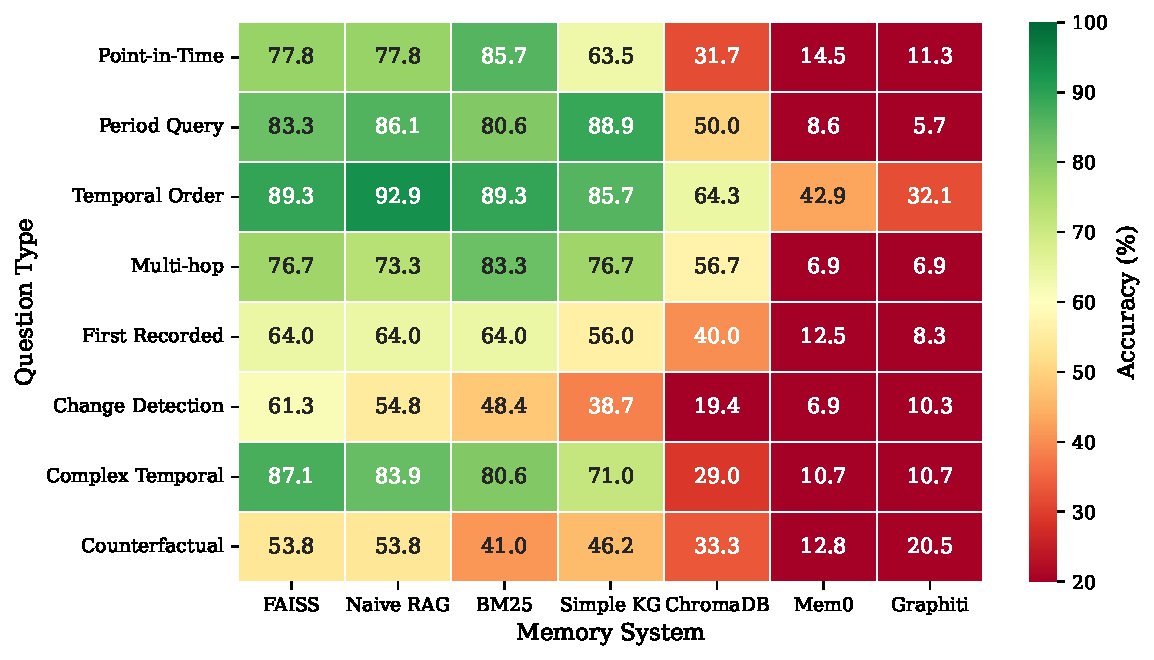
\includegraphics[width=\columnwidth]{figures/fig3_heatmap.pdf}
\caption{System $\times$ question type accuracy heatmap. No single system dominates all types; the 40.6pp spread across types confirms the typology captures distinct challenges.}
\label{fig:heatmap}
\end{figure}

Figure~\ref{fig:heatmap} reveals substantial system$\times$type interactions.
FAISS leads on complex temporal (87.1\%) and counterfactual (53.8\%); BM25 excels at point-in-time (85.7\%) and multi-hop (83.3\%); Simple KG tops period query (88.9\%).
The 40.6pp spread across question types (counterfactual: 48.7\% to temporal order: 89.3\%) validates the typology.

\subsection{Difficulty Calibration}
All five systems show monotonic L1$\to$L3 degradation, but with strikingly different robustness: FAISS drops only 2.9pp vs.\ BM25's 16.6pp (Figure~\ref{fig:difficulty}).
FAISS's dense representations appear to maintain semantic relevance even under complex compositional demands, while BM25's keyword matching deteriorates sharply when query--document lexical overlap decreases.

\begin{figure}[t]
\centering
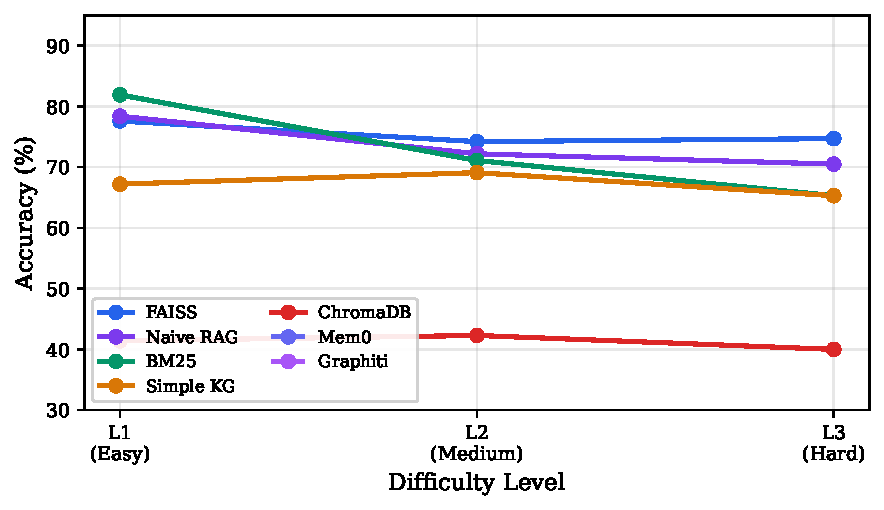
\includegraphics[width=\columnwidth]{figures/fig4_difficulty.pdf}
\caption{Accuracy degradation from L1 to L3. FAISS is most robust ($-$2.9pp); BM25 is most fragile ($-$16.6pp).}
\label{fig:difficulty}
\end{figure}

\subsection{System Complementarity}
An oracle ensemble (correct if \emph{any} system answers correctly) achieves \textbf{85.4\%}, a 9.8pp gain over the best single system, confirming that memory backends have substantially non-overlapping error profiles (Figure~\ref{fig:complementarity}).
FAISS-ChromaDB Jaccard overlap is only 0.446 (lowest), while FAISS-SimpleKG is 0.746.
Simple KG uniquely solves 6 items that FAISS misses, and ChromaDB uniquely solves 6, despite its low overall accuracy.
45 items (14.6\%) are answered incorrectly by \emph{all} systems, establishing a hard irreducible ceiling.

\begin{figure}[t]
\centering
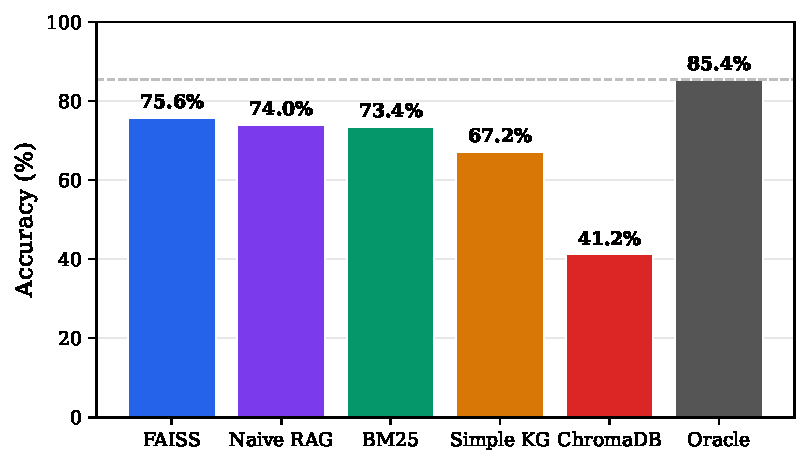
\includegraphics[width=\columnwidth]{figures/fig5_complementarity.pdf}
\caption{Oracle ensemble reaches 85.4\% vs.\ 75.6\% best single system. 45 irreducible failures suggest retrieval-independent challenges.}
\label{fig:complementarity}
\end{figure}

\subsection{Cross-Benchmark Validation with LoCoMo}
Table~\ref{tab:locomo} compares BiTempQA results with LoCoMo evaluation.
The most striking finding is Simple KG's asymmetry: 97.5\% adversarial accuracy on LoCoMo (best of all systems, +34pp above average) but 37.5\% temporal reasoning on LoCoMo (worst, $-$9pp) and 67.2\% on BiTempQA.
This reflects a fundamental trade-off: graph structures resist adversarial hallucination (returning empty context for non-existent facts) but lack the retrieval breadth needed for temporal reasoning.

\begin{table}[t]
\centering
\resizebox{\columnwidth}{!}{%
\begin{tabular}{lccccc}
\toprule
& \multicolumn{2}{c}{\textbf{BiTempQA}} & \multicolumn{3}{c}{\textbf{LoCoMo}} \\
\cmidrule(lr){2-3} \cmidrule(lr){4-6}
\textbf{System} & Overall & Temporal & Overall & Temporal & Adversarial \\
\midrule
FAISS & \textbf{75.6\%} & \textbf{75.6\%} & \textbf{57.0\%} & \textbf{46.9\%} & 63.0\% \\
Naive RAG & 74.0\% & 74.0\% & 54.4\% & 42.7\% & 69.7\% \\
BM25 & 73.4\% & 73.4\% & 55.8\% & 43.8\% & 64.8\% \\
Simple KG & 67.2\% & 67.2\% & 56.8\% & 37.5\% & \textbf{97.5\%} \\
\bottomrule
\end{tabular}%
}
\caption{Cross-benchmark comparison. Simple KG shows extreme adversarial-temporal asymmetry.}
\label{tab:locomo}
\end{table}

\section{Diagnostic Analysis}

\subsection{Retrieval Is the Bottleneck}
% 中文注释：这里改成更短的表达，同时顺手消除开头那条轻微的断行 warning。
We sampled 20 FAISS failures and grouped them by retrieval-context length.
% 中文注释：这里只统一符号间距和普通字体，不改变分析结论。
All 20 had short or empty retrieval context ($< 200$ characters), compared with an average of $\sim 500$ characters for correct answers.
This heuristic analysis attributes roughly $\sim 55\%$ of the sampled failures to retrieval and $\sim 45\%$ to downstream reasoning, suggesting that improvements in retrieval quality, particularly temporal-aware retrieval, may yield larger gains than improvements in reasoning alone.

\subsection{Confidence Is Anti-Calibrated}
% 中文注释：保留术语，但取消不必要的斜体强调，让正文更接近 ACL 常见风格。
A notable diagnostic finding is that some vector-based systems exhibit anti-calibrated confidence scores.
Table~\ref{tab:calibration} shows Expected Calibration Error (ECE), Brier score, and AUROC for each system.

\begin{table}[t]
\centering
\small
\begin{tabular}{lccc}
\toprule
\textbf{System} & \textbf{ECE}$\downarrow$ & \textbf{Brier}$\downarrow$ & \textbf{AUROC} \\
\midrule
FAISS & 0.163 & 0.229 & 0.453 \\
Naive RAG & 0.319 & 0.303 & 0.552 \\
BM25 & 0.235 & 0.769 & 0.467 \\
Simple KG & 0.672 & 0.672 & 0.500 \\
ChromaDB & 0.412 & 0.412 & 0.500 \\
\bottomrule
\end{tabular}
\caption{Confidence calibration metrics. FAISS and BM25 show AUROC $< 0.5$, meaning that wrong answers receive higher confidence than correct ones.}
\label{tab:calibration}
\end{table}

FAISS's AUROC of 0.453 indicates that confidence scores are worse than random at predicting correctness: wrong answers often receive higher confidence than correct ones.
This has practical implications, because agents cannot reliably use internal confidence alone to determine whether a temporal-memory answer should be trusted or externally verified.

\subsection{Knowledge Retraction vs.\ Version Tracking}
We decompose performance on questions involving knowledge dynamics (Table~\ref{tab:retraction}).
Simple KG shows an asymmetric profile: it is relatively strong on version tracking (81.0\%, close to FAISS's 82.8\%) but weaker on knowledge retraction (53.6\%).
This pattern suggests that graph structures may naturally support tracking fact evolution, while handling explicit revocation of superseded knowledge remains more difficult.

\begin{table}[t]
\centering
% 中文注释：该表继续保持按栏宽缩放，只统一字体和符号间距，不改变尺寸策略。
\resizebox{\columnwidth}{!}{%
\begin{tabular}{lccc}
\toprule
\textbf{System} & \textbf{Retraction (28Q)} & \textbf{Ver.\ Track.\ (58Q)} & \textbf{Neither (222Q)} \\
\midrule
FAISS & 67.9\% & \textbf{82.8\%} & 74.8\% \\
Naive RAG & 67.9\% & 75.9\% & 74.3\% \\
BM25 & 57.1\% & 74.1\% & \textbf{75.2\%} \\
Simple KG & 53.6\% & 81.0\% & 65.3\% \\
ChromaDB & 39.3\% & 37.9\% & 42.3\% \\
\bottomrule
\end{tabular}%
}
\caption{Accuracy by knowledge-dynamics type. Simple KG is strong at version tracking but weak at retraction. Bootstrap CIs for retraction span 35pp because $n = 28$ is small.}
\label{tab:retraction}
\end{table}

\subsection{Implications for Memory System Design}
Our findings suggest three design implications:

\paragraph{1. Temporal-aware retrieval.}
Since $\sim 55\%$ of sampled failures are retrieval-limited, adding temporal metadata filtering (e.g., ``retrieve only facts recorded before $T$'') or bitemporal indexing may yield larger gains than improving the reasoning model alone.

\paragraph{2. Hybrid vector+graph architectures.}
% 中文注释：这里只统一字体，不改原始推断力度。
The complementarity between systems (oracle +9.8pp) and Simple KG's adversarial robustness suggest that combining dense retrieval's breadth with graph structure's precision could outperform either approach alone.

\paragraph{3. External verification for temporal claims.}
Anti-calibrated confidence means that internal signals are unreliable for identifying uncertain temporal answers. External verification, such as cross-checking against source timestamps, may therefore be especially valuable for bitemporal queries.

\section{Conclusion}

We presented BiTempQA, the first diagnostic benchmark explicitly designed to evaluate bitemporal reasoning (reasoning about \emph{when events occurred} vs.\ \emph{when the system learned about them}) in LLM agent memory systems.
Our evaluation of five memory backends reveals three key findings.

First, \textbf{record-time reasoning is genuinely harder} than event-time reasoning ($p{=}0.023$), confirming that the dual-timestamp distinction captures a real cognitive challenge.
Second, \textbf{retrieval, not reasoning, is the primary bottleneck} (${\sim}55\%$ of failures), suggesting that temporal-aware retrieval mechanisms would yield the largest improvements.
Third, \textbf{memory backends are highly complementary}: an oracle ensemble achieves 85.4\% (+9.8pp), and graph-based memory offers unique adversarial robustness (97.5\%) despite lower temporal accuracy.

These findings provide actionable guidance for building temporally-aware memory systems: invest in bitemporal indexing, combine vector breadth with graph precision, and use external verification rather than internal confidence.

Future work includes: human expert validation, English translation, evaluation of production memory systems (Mem0, Graphiti, TMG), and expansion to longer scenarios with richer temporal dynamics.

% 中文注释：按 ACL 官方格式要求，将 Limitations 放在 Conclusion 之后、References 之前。
\section{Limitations}
\label{sec:limitations}

We acknowledge several limitations:

\paragraph{Scale and language.}
BiTempQA v3 contains 415 items (84 test) in Chinese only. While sufficient for diagnostic analysis, the small test set limits the granularity of per-type breakdowns (e.g., only 4 scenario types appear in the test set). Expanding the test set and adding English translations are priorities for future work.

\paragraph{Short-context scenarios only.}
Current scenarios contain 2--7 memory writes each, reflecting the length of ChronoQA golden chunks and curated event descriptions.
This limits our ability to test retrieval selectivity under longer contexts (50+ writes), where retrieval design may become a stronger differentiator.
The tight clustering of top systems (81.0--82.1\%) may not hold for longer scenarios.

\paragraph{Test set composition.}
The test set consists entirely of real-source scenarios and covers only 4 of 10 scenario types (entity attribute evolution, multi-source information, relationship evolution, temporal ambiguity).
The remaining 6 types are represented only in the training set via LLM-generated scenarios.

\paragraph{Abstractive-only evaluation.}
All test questions use abstractive (free-text) answers evaluated by LLM judge.
LLM judge leniency may inflate accuracy relative to human evaluation.

\paragraph{Production system LLM confound.}
Mem0 and Graphiti use Qwen2.5-32B-Instruct as their internal LLM for memory extraction, while lightweight backends use DeepSeek-V3 for answer generation.
Their low scores (2--8\%) therefore reflect a combination of architectural limitations (memory compression, lack of bitemporal indexing) and LLM integration challenges.
Evaluating with a fully compatible LLM backend may yield higher absolute scores, though we expect the qualitative patterns---compressed memories losing temporal detail---to persist.

\paragraph{ChromaDB interpretation.}
While ChromaDB uses the same embedding model as other vector systems, its metadata filtering approach is architecturally distinct from pure similarity search. Its 22.6\% accuracy reflects the interaction between metadata filtering and heterogeneous temporal formats, not necessarily a fundamental limitation of vector databases.

% 中文注释：按 ACL 官方建议，将 Ethics Statement 放在 Conclusion/Limitations 之后、References 之前。
\section{Ethics Statement}

% 中文注释：伦理说明保持简短克制，只统一正文字体和少量符号间距，不增加新的内容主张。
BiTempQA is intended as an evaluation benchmark for memory systems rather than as a deployed decision-making tool. The dataset is generated from synthetic scenarios and does not intentionally include private personal data. This design reduces direct privacy risk, but it does not eliminate the possibility that generated examples may still reflect cultural, linguistic, or model-induced biases.

% 中文注释：这里保持与 limitations 一致，只去掉多余的样式感。
Our experiments also rely on LLM-generated QA pairs and an LLM-based judge. As discussed in the limitations section, this introduces risks of annotation noise, judge leniency, and benchmark artifacts. We therefore view the benchmark as a diagnostic instrument for controlled comparison rather than as a definitive measure of real-world temporal reliability.

% 中文注释：最后一段继续保持 EMNLP 风格的克制表述。
We recommend that future releases include human validation, broader linguistic coverage, and additional checks for harmful stereotypes or misleading temporal claims. Any use of the benchmark to evaluate production systems in sensitive domains should be accompanied by task-specific safety review and external verification.


% 中文注释：EMNLP/ACL 模板的 acl.sty 已经内置 bibliographystyle，这里只保留 bibliography。
% 中文注释：references.bib 中的条目已按会议论文 / arXiv / 官网资源分别做了兼容 BibTeX 的格式整理。
\bibliography{references}

\appendix
\section{Appendix}

\subsection{Full Per-Question-Type Results}

Table~\ref{tab:full_qtype} provides complete per-question-type accuracy across all systems and types.

\begin{table*}[h]
\centering
\footnotesize
\setlength{\tabcolsep}{4pt}
\begin{tabular}{lccccc}
\toprule
\textbf{Question Type (Level)} & \textbf{FAISS} & \textbf{BM25} & \textbf{Naive RAG} & \textbf{Simple KG} & \textbf{ChromaDB} \\
\midrule
Point-in-Time (L1) & 77.8\% & \textbf{85.7\%} & 77.8\% & 63.5\% & 31.7\% \\
Temporal Order (L1) & 89.3\% & 89.3\% & \textbf{92.9\%} & 85.7\% & 64.3\% \\
First Recorded (L1) & 64.0\% & 64.0\% & 64.0\% & 56.0\% & 40.0\% \\
Period Query (L2) & 83.3\% & 80.6\% & \textbf{86.1\%} & 88.9\% & 50.0\% \\
Change Detection (L2) & \textbf{61.3\%} & 48.4\% & 54.8\% & 38.7\% & 19.4\% \\
Multi-hop Temporal (L2) & 76.7\% & \textbf{83.3\%} & 73.3\% & 76.7\% & 56.7\% \\
Counterfactual (L3) & \textbf{53.8\%} & 41.0\% & 53.8\% & 46.2\% & 33.3\% \\
Complex Temporal (L3) & \textbf{87.1\%} & 80.6\% & 83.9\% & 71.0\% & 29.0\% \\
\midrule
\textbf{Average} & \textbf{74.2\%} & 71.5\% & 72.2\% & 65.8\% & 40.7\% \\
\bottomrule
\end{tabular}
\caption{Complete per-question-type accuracy. Version Conflict excluded due to insufficient samples. Spread: 48.7\% (Counterfactual) to 92.9\% (Temporal Order).}
\label{tab:full_qtype}
\end{table*}

\subsection{LLM Judge Cross-Validation Details}

We cross-validated DeepSeek-V3 against Qwen2.5-72B-Instruct on 50 abstractive QA pairs from the FAISS system (random sample, seed=42).

\begin{table}[h]
\centering
\small
\begin{tabular}{lc}
\toprule
\textbf{Metric} & \textbf{Value} \\
\midrule
Agreement rate & 76.0\% (38/50) \\
Cohen's $\kappa$ & 0.455 (moderate) \\
DeepSeek-V3 judged correct & 80.0\% (40/50) \\
Qwen2.5-72B judged correct & 60.0\% (30/50) \\
\midrule
\multicolumn{2}{l}{\textit{Disagreement breakdown (12 items)}} \\
\quad DeepSeek lenient & 11/12 (91.7\%) \\
\quad Qwen lenient & 1/12 (8.3\%) \\
\quad Pattern: partial answer & 6/12 \\
\quad Pattern: answer too short & 6/12 \\
\bottomrule
\end{tabular}
\caption{LLM Judge cross-validation. DeepSeek-V3 is systematically more lenient, accepting partial answers that Qwen rejects.}
\label{tab:judge_detail}
\end{table}


\end{document}
